\chapter{Overview}
\label{storage}

\section{Components}
\label{storage:components}

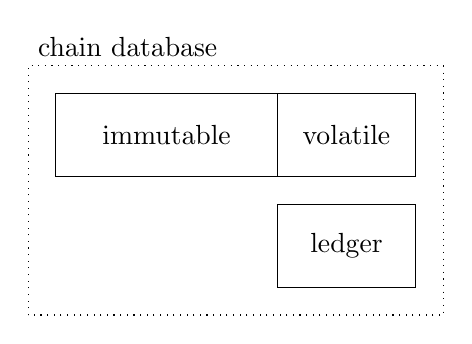
\begin{tikzpicture}
\draw [dotted]
     (-50pt, -65pt)
  -- ++(0, 90pt) node[above right] {chain database}
  -- ++(150pt, 0)
  -- ++(0, -90pt)
  -- cycle;
\node [draw, shape=rectangle, minimum width=80pt, minimum height=30pt] at (0,0)  {immutable};
\node [draw, shape=rectangle, minimum width=50pt, minimum height=30pt] at (65pt, 0)  {volatile};
\node [draw, shape=rectangle, minimum width=50pt, minimum height=30pt] at (65pt, - 40pt) {ledger};
\end{tikzpicture}

Discuss the immutable/volatile split (we reference this section for that).

\section{In memory}
\label{storage:inmemory}

TODO: After we discussed the overview, we should give an overview of everything
we store in memory in any component, so that we have a better understanding of
memory usage of the chain DB as a whole.

\subsection{Resource registry}
\label{storage:resourceregistry}

In order to deal with resource allocation and deallocation, we use the
abstraction of the \lstinline!ResourceRegistry!. The resource registry is a
generalization of the \lstinline!bracket! pattern. Using a bracket imposes strict
rules on the scope of the allocated variables, as once the body of the
\lstinline!bracket! call finishes, the resources will be deallocated.

On some situations this is too constraining and resources, despite the need to
ensure they are deallocated, need to live for longer periods or be shared by
multiple consumers. The registry itself lives in a \lstinline!bracket!-like
environment, but the resources allocated in it can be opened and closed at any
point in the lifetime of the registry and will ultimately be closed when the
registry is being closed if they are still open at that time.

The allocation function for a given resource will run with exceptions
unconditionally masked, therefore on an uninterruptible fashion. Because of
this, it is important that such functions are fast. Note that once the
allocation call finishes, the resource is now managed by the registry and will
be deallocated in case an exception is thrown.

A resource that is allocated will be returned coupled with its
\lstinline!ResourceKey! that can be used to release the resource as it holds a
reference to the registry in which it is allocated.

Special care has to be put when resources are dependent one to another. For
example, a thread allocated in the registry might hold some mutable reference to
a file handle that is replaced at certain points during the execution. In such
cases, the sequence of deallocation must take this into account and deallocate
the resources in reverse order of dependency.

Also when deallocating the resources, we must ensure that the right order of
deallocation is preserved. Right order here means that as resources that were
allocated later than others could potentially use the latter, the later ones
should probably be deallocated before the earlier ones (unless otherwise taken
care of). Resources in the registry are indexed by their \emph{age} which is a
meaningless backwards counter. A resource is considered older than another if
its age is greater than the one of the other resource. Conversely, a resource is
considered younger if the opposite holds.

\subsubsection{Temporary registries}
\label{storage:temporaryregs}

When some resources are not meant to be directly allocated in a registry, one
can take advantage of temporary resource registries as a temporary container for
those resources. For this purpose, the \lstinline!WithTempRegistry! is made
available. It is basically a \lstinline!StateT! computation which will check
that the resource was indeed transferred properly to the returned value and then
the registry will vanish.

Using this construction will ensure that if an exception is thrown while the
resources are being allocated but before they are kept track by the resulting
state, they will be released as the registry itself will close in presence of an
exception. Note that once the resource was transferred to the final state, no
more tracking is performed and the resource could be leaked. It is then
responsibility of the resulting state to eventually deallocate the resource.

Temporary registries are useful when we want to run localized allocations and
checks, i.e. allocations and checks that use implementation details that should
remain hidden for upper layers. Specially this is useful when we expect to run a
computation that will provide a result that holds some API which references some
internal data types which are not directly accessible from the API, but we still
want to run some checks on those internal data types. \footnote{See
  \lstinline!VolatileDB.openDB! for an example. The inner computation allocates
  and performs checks against a \lstinline!OpenState blk h! wereas the returned
  value is a \lstinline!VolatileDB! which has a \lstinline!close! function but
  otherwise has no direct access to the internal \lstinline!OpenState blk h!.}
The resulting value will be transitively closable from the general registry
through functions on the API (deallocating its resources), but the actual value
is not accessible to perform checks.

Note that if we just run the inner computation and return the API value, there
is a short time span during which an exception would leak the resources as the
API that can close the resources is not yet included in any exception handler
that will close it. A special case of this situation is when we run a
computation with a (\emph{upper}) registry and we want to perform a localized
allocation and checks on an internal component. The combinator
\lstinline!runInnerWithTempRegistry! is provided. This combinator will make sure
that the resources are allocated in the \emph{upper} registry before closing the
inner one (therefore performing the allocation checks against the resulting
inner state), and thus in presence of an exception the resources will be safely
deallocated. There are a couple of subtleties here that are worth being
mentioned:

\begin{itemize}
  \item There is a short time span during which the inner registry has not yet
        vanished, but the resource has already been allocated in the greater
        registry. An exception in this exact moment will lead to double freeing
        a resource.
  \item Unless the greater resulting state has some way of accessing the
        returned inner state, the function that performs the checks will
        necessarily be trivial (i.e. \lstinline!const (const True)!). If we had
        a way to access the inner returned state, we could run the checks, but
        adding this implies leaking the inner state, its representation and
        functions, and most of the times this is not desirable as those are
        usually private implementation details.
\end{itemize}

\paragraph{Specialization to \lstinline!TrackingTempRegistry!} The
\lstinline!TempRegistry! concept could be specialized in a narrower concept, a
\lstinline!TrackingTempRegistry! which would essentially be equivalent to a
\lstinline!TempRegistry () m! and no checks would be preformed on the resulting
state. This way some redundant situations could be simplified. Note that this is
also equivalent to using a normal \lstinline!ResourceRegistry! which leaks all
the allocated resources when going out of scope.

\subsection{Chain fragments}
\label{storage:fragments}

\subsection{Extended ledger state}
\label{storage:extledgerstate}
\label{storage:headerstate}

TODO: Is there a more natural place to talk about this? Introducing the
header state when introducing the storage layer does not feel quite right.
The storage layer might be storing the header state, but that doesn't
explain its existence.

ChainDepState, (ChainIndepState), LedgerState, ExtLedgerState
